\let\lesson\undefined
\newcommand{\lesson}{\phantomlesson{Bài 10.}}
\setcounter{section}{2}
\section{Bài tập trắc nghiệm}
\begin{enumerate}[label=\bfseries Câu \arabic*:]
	\item \mkstar{1}\\
	{Điều nào sau đây là sai khi nói về sự tương tác giữa các vật?
		\begin{mcq}
			\item Tác dụng giữa các vật bao giờ cũng có tính chất hai chiều (gọi là tương tác).
			\item Tác dụng giữa các vật bao giờ cũng có tính chất hai chiều (gọi là tương tác).
			\item Khi vật A tác dụng lên vật B thì ngược lại, vật B cũng tác dụng ngược lại vật A.
			\item Khi vật A tác dụng lên vật B thì chỉ có vật B thu gia tốc, còn vật A thì không.
		\end{mcq}
	
}
\hideall{
\textbf{Đáp án: D.}
}

\item\mkstar{1}\\
{Cặp "lực và phản lực" trong định luật III Newton
	\begin{mcq}
		\item tác dụng vào cùng một vật.
		\item tác dụng vào hai vật khác nhau.
		\item không bằng nhau về độ lớn.
		\item bằng nhau về độ lớn nhưng không cùng giá.
	\end{mcq}

}
\hideall{
\textbf{Đáp án: B.}
}

\item\mkstar{2}\\
{Người ta dùng búa đóng một cây đinh vào một khối gỗ thì
	\begin{mcq}
		\item lực của búa tác dụng vào đinh lớn hơn lực đinh tác dụng vào búa.
		\item lực của búa tác dụng vào đinh về độ lớn bằng lực của đinh tác dụng vào búa.
		\item lực của búa tác dụng vào đinh nhỏ hơn lực đinh tác dụng vào búa.
		\item tùy thuộc đinh di chuyển nhiều hay ít mà lực do đinh tác dụng vào búa lớn hơn hay nhỏ hơn lực do búa tác dụng vào đinh.
	\end{mcq}

}
\hideall{
\textbf{Đáp án: B.}
}

\item \mkstar{2}\\
{Khi một con ngựa kéo xe, lực tác dụng vào con ngựa làm cho nó chuyển động về phía trước là
	\begin{mcq}(2)
		\item lực mà con ngựa tác dụng vào xe.
		\item lực mà xe tác dụng vào ngựa.
		\item lực mà ngựa tác dụng vào đất.
		\item lực mà đất tác dụng vào ngựa.
	\end{mcq}

}
\hideall{
\textbf{Đáp án: D.}
}

\item \mkstar{2}\\
{Điều khẳng định nào sau đây là đúng?   
	\begin{mcq}
		\item Lực hấp dẫn do Trái Đất tác dụng lên cơ thể bạn thì nhỏ hơn lực hấp dẫn do bạn tác dụng lên Trái Đất vì khối lượng của bạn nhỏ hơn khối lượng của Trái Đất.  
		\item Mặt Trăng quay quanh Trái Đất vì Trái Đất tác dụng lực hấp dẫn lên Mặt Trăng và Mặt Trăng cũng tác dụng một lực hấp dẫn lên Trái Đất cùng độ lớn và cùng hướng.  
		\item Khi tên lửa bắt đầu được phóng lên từ Trái Đất thì nó tác dụng một lực lên Trái Đất bằng với lực do Trái Đất tác dụng lên nó.  
		\item Một chiếc máy bay đang bay với tốc độ không đổi thì không chịu tác dụng của trọng lực.
	\end{mcq}

}
\hideall{
\textbf{Đáp án: C.}
}

\item\mkstar{2}\\
{Hai đội chơi đang tham gia trò chơi kéo co thì sợi dây đột nhiên bị đứt. Điều gì sẽ xảy ra ngay sau đó?   
	\begin{mcq}
		\item Vì lực tác dụng của hai đội không bằng nhau nên hai đội sẽ bị chuyển động về hướng của đội kéo mạnh hơn.  
		\item Lực do người chơi tác dụng không còn cân bằng với lực căng dây nên các đội sẽ bị tăng tốc theo các hướng ngược lại.  
		\item Trọng lực cân bằng với lực do người tác dụng nên các đội sẽ bị ngã xuống.  
		\item Lực căng của sợi dây kéo các đội tăng tốc theo các hướng ngược nhau.   
	\end{mcq}

}
\hideall{
\textbf{Đáp án: B.}
}

\item\mkstar{2}\\
{Một chiếc tàu đang chuyển động trên sông. Trong một khoảng thời gian nào đó, tàu đang chuyển động thẳng đều và giả sử rằng trên phương nằm ngang tàu chỉ chịu tác dụng bởi lực đẩy của động cơ và lực cản của nước thì nhận xét nào sau đây là đúng?   
	\begin{mcq}
		\item Lực đẩy của động cơ có độ lớn nhỏ hơn lực cản của nước.  
		\item Lực đẩy của động cơ và lực cản của nước cùng cùng phương và cùng chiều.  
		\item Lực đẩy của động cơ có độ lớn lớn hơn lực cản của nước.  
		\item Lực đẩy của động cơ và lực cản của nước là hai lực trực đối. 
	\end{mcq}

}
\hideall{
\textbf{Đáp án: D.}
}

\item\mkstar{2}\\
{Khẳng định nào sau đây về lực và phản lực là đúng?
	\begin{mcq}
		\item Khẳng định nào sau đây về lực và phản lực là đúng?
		\item Lực và phản lực xuất hiện đồng thời và cùng tác dụng vào một vật.
		\item Lực và phản lực là hai lực cùng hướng và cùng độ lớn.
		\item Lực và phản lực là xuất hiện khi có sự tương tác giữa hai vật.
	\end{mcq}

}
\hideall{
\textbf{Đáp án: D.}
}

\item\mkstar{2}\\
{Chọn phát biểu đúng trong các phát biểu sau:\\
	Trong khi chơi bóng chày, quả bóng của Nobita đã đập vỡ cửa kính của nhà bác hàng xóm. 
	\begin{mcq}
		\item Lực do quả bóng tác dụng vào cửa kính (về độ lớn) lớn hơn lực do của kính tác dụng vào quả bóng.
		\item Lực do quả bóng tác dụng vào cửa kính (về độ lớn) nhỏ hơn lực do cửa kính tác dụng vào quả bóng.
		\item Lực do quả bóng tác dụng vào cửa kính (về độ lớn) bằng lực do cửa kính tác dụng vào quả bóng.
		\item Lực do quả bóng tác dụng vào cửa kính (về độ lớn) lớn hơn trọng lực của cửa kính.
	\end{mcq}

}
\hideall{
\textbf{Đáp án: C.}
}

\item \mkstar{2}\\
{Khi nói về sự tương tác giữa hai vật, điều nào sau đây là sai?
	\begin{mcq}
		\item Tác dụng giữa hai vật bao giờ cũng có tính chất hai chiều.
		\item Khi một vật chuyển động có gia tốc thì chứng tỏ đã có lực tác dụng lên vật.
		\item Khi A và B tương tác với nhau thì gia tốc mà hai vật thu được luôn có cùng độ lớn.
		\item Lực tác dụng và phản lực tác dung luôn xuất hiện và mất đi đồng thời.
	\end{mcq}

}
\hideall{
\textbf{Đáp án: C.}
}

\item\mkstar{3}\\
{Một quả bóng bay đến đập vào tường, sau đó quả bóng bị bật ngược trở lại còn tường thì vẫn đứng yên. Điều khẳng định nào sau đây là đúng?
	\begin{mcq}
		\item Quả bóng chịu tác dụng của phản lực do tường tác dụng lên quả bóng nhưng tường không chịu tác dụng lực của quả bóng tác dụng lên nó.
		\item Phản lực do tường tác dụng lên quả bóng thì lớn hơn nhiều so với lực do quả bóng tác dụng vào tường vì khối lượng của quả bóng rất nhỏ.
		\item Phản lực do tường tác dụng lên quả bóng và lực do quả bóng tác dụng lên tường có cùng độ lớn nhưng vì khối lượng của tường quá lớn nên gia tốc tường thu được vô cùng bé.
		\item Khi chạm vào tường, quả bóng bị bật ngược trở lại do quán tính, còn tường vẫn đứng yên vì nó có xu hướng bảo toàn trạng thái đứng yên.
	\end{mcq}

}
\hideall{
\textbf{Đáp án: C.}
}

\item\mkstar{3}\\
{Một chiếc ô tô đâm vào bức tường, điều khẳng định nào sau đây là đúng?
	\begin{center}
		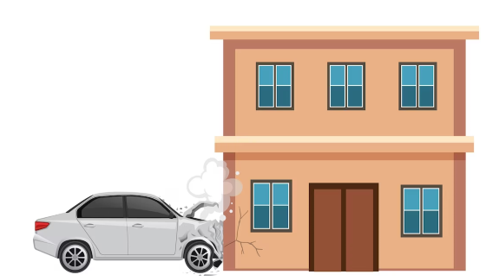
\includegraphics[width=0.4\linewidth]{../figs/VN10-2023-PH-TP017-P-1}
	\end{center}
\begin{mcq}
	\item Lực do ô tô tác dụng vào tường lớn hơn lực do tường tác dụng vào ô tô.
	\item Lực do ô tô tác dụng vào tường bằng lực do tường tác dụng vào ô tô.
	\item Lực do ô tô tác dụng vào tường nhỏ hơn lực do tường tác dụng vào ô tô.
	\item Lực do ô tô tác dụng vào tường bằng 0, lực do tường tác dụng vào ô tô thì khác 0.
\end{mcq}
}
\hideall{
\textbf{Đáp án: B.}
}
\end{enumerate}
\section{Bài tập tự luận}
\begin{enumerate}[label=\bfseries Bài \arabic*:]
	\item \mkstar{1}
	
	{
		Một vật đang nằm yên trên mặt bàn nằm ngang. Tại sao ta có thể khẳng định rằng bàn đã tác dụng một lực lên nó?
	}
	
	\hideall{
		
		Giả sử mặt bàn không tác dụng lực lên nó thì vật đó chỉ chịu tác dụng của lực hút trái đất. Thì nó sẽ bị kéo về hướng lực hút trái đất tức là nó sẽ bị rơi khỏi mặt bàn. vậy nên khi vật đang nằm yên trên bàn và không bị rớt ra khỏi bản thì ngoài lực hút trái đất thì nó còn phải chịu một lực khác nữa để cân bằng với lực hút trái đất. Đó chính là lực đỡ của mặt bàn.
	}


\item \mkstar{1}

{
	Hãy chỉ ra các cặp lực và phản lực trong hai trường hợp sau:
	\begin{enumerate}[label=\alph*)]
		\item Quyển sách nằm yên trên mặt bàn hình a.
		\item Dùng búa đóng đinh vào gỗ hình b.
	\end{enumerate}
	\begin{center}
		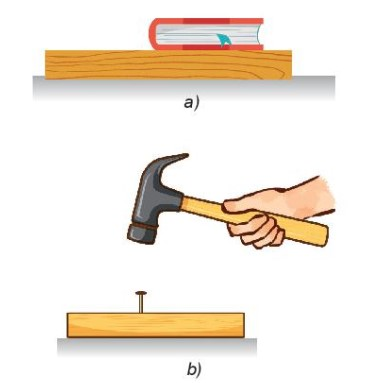
\includegraphics[scale=0.7]{../figs/VN10-2022-PH-TP017-3.jpg}
	\end{center}
}

\hideall{
	\begin{enumerate}[label=\alph*)]
		\item Lực là áp lực gây ra bởi trọng lực của vật tác dụng lên bàn, phản lực là lực nâng (phản lực đàn hồi) của mặt bàn tác dụng lên vật.\\
		Có thể kể thêm: Lực là lực hấp dẫn do Trái Đất tác dụng lên vật, phản lực là lực hấp dẫn do vật tác dụng lên Trái Đất.
		\item Lực do búa tác dụng lên đinh và phản lực của đinh tác dụng vào búa.
	\end{enumerate}
}
\item \mkstar{1}

{
	
	Một ô tô chuyển động trên mặt đường, nếu lực do ô tô tác dụng lên mặt đường có độ lớn bằng lực mà mặt đường đẩy ô tô thì tại sao chúng không "khử nhau"?
	\begin{center}
		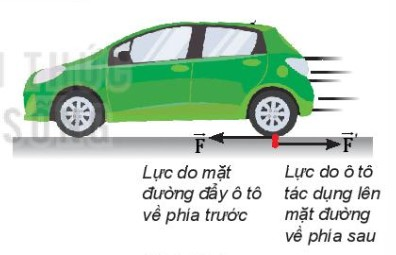
\includegraphics[scale=0.6]{../figs/VN10-2022-PH-TP017-4.jpg}
	\end{center}
}

\hideall{
	
	Vì căn bản 2 lực này tác dụng lên hai vật khác nhau. Lực do ô tô tác dụng lên mặt đường thì lực được đặt ở mặt đường. Lực mà mặt đường đẩy ô tô thì được đặt vào ô tô.
}



	\item \mkstar{2}\\
	{Hai người kéo một sợi dây theo hai hướng ngược nhau, mỗi người kéo một lực $\SI{50}{\newton}$. Hỏi sợi dây có bị đứt hay không nếu nó chỉ chịu được lực căng tối đa là $\SI{70}{\newton}$?
	
}
\hideall{
Lực căng của dây $F=\SI{50}{\newton}<\SI{70}{\newton}$ nên dây không đứt.
}

\item\mkstar{2}\\
{Hai bạn Bình và An cầm hai đầu một sợi dây và kéo căng thì sợi dây không bị đứt, nhưng nếu buộc một đầu sợi dây đó vào gốc cây và hai bạn cùng kéo căng một đầu sợi dây thì đây đứt. Hãy giải thích tại sao.

}
\hideall{
Khi Bình và An cầm hai đầu một sợi dây rồi kéo căng thì hai đầu dây chịu tác dụng của hai lực cân bằng nhau $\overrightarrow{F}$ và $-\overrightarrow{F}$, rồi lực căng của dây bằng $F$ nên dây không bị đứt. Khi hai người cầm chung một đầu dây mà kéo, đầu kia buộc vào thân cây, thì hai người đã tác dụng vào dây một lực gấp đôi là $2F$. Dây sẽ truyền lực $2F$ đó tới cây. Theo định luật III Newton, cây cũng tác dụng trở lại dây một phản lực có độ lớn $2F$. Vậy, hai đầu dây bị kéo về 2 phía với lực lớn gấp đôi trường hợp trước, vì thế mà dây dễ bị đứt.
}

\item\mkstar{3}\\
{Một vật khối lượng $\SI{1}{\kilogram}$ chuyển động về phía trước với vận tốc $\SI{5}{\meter/\second}$ va chạm vào một vật thứ hai đang đứng yên. Sau va chạm vật thứ nhất chuyển động ngược trở lại với vận tốc $\SI{1}{\meter/\second}$. Còn vật thứ hai chuyển động với vận tốc $\SI{2}{\meter/\second}$. Xác định khối lượng của vật thứ hai.

}
\hideall{
$m_2=\SI{3}{\kilogram}$.
}

\item \mkstar{3}\\
{Một quả bóng khối lượng $\SI{200}{\gram}$ bay với vận tốc $\SI{72}{\kilo\meter/\hour}$ đến đập vuông góc vào tường rồi bật trở lại theo phương cũ với vận tốc $\SI{54}{\kilo\meter/\hour}$. Thời gian va chạm giữa bóng và tường là $\SI{0.05}{\second}$. Xác định độ lớn lực của tường tác dụng lên quả bóng.

}
\hideall{
$F=\SI{140}{\newton}$.
}

\item \mkstar{3}\\
{Một viên bi A có khối lượng $m_A=\SI{300}{\gram}$ đang chuyển động với vận tốc $\SI{3}{\meter/\second}$ thì va chạm với viên bi B có khối lượng $m_B=2m_A$ đang đứng yên trên mặt bàn nhẵn, nằm ngang. Biết sau thời gian va chạm, viên bi B chuyển động với vận tốc $\SI{0.5}{\meter/\second}$ cùng chiều chuyển động ban đầu của viên bi A. Bỏ qua mọi ma sát, tính vận tốc chuyển động của viên bi A ngay sau va chạm.

}
\hideall{
$v_A=\SI{2}{\meter/\second}$.
}
\end{enumerate}